\part{运动产生}
\markboth{运动产生}{运动产生}

\chapter{肌肉生物学和力量}\label{chap:chap4}


孤身一人,我们能做的太少。
团结起来,我们能做的却很多。
\begin{flushright}
	————海伦$\cdot$凯勒
\end{flushright}


\begin{figure}[!htb]
	\centering
	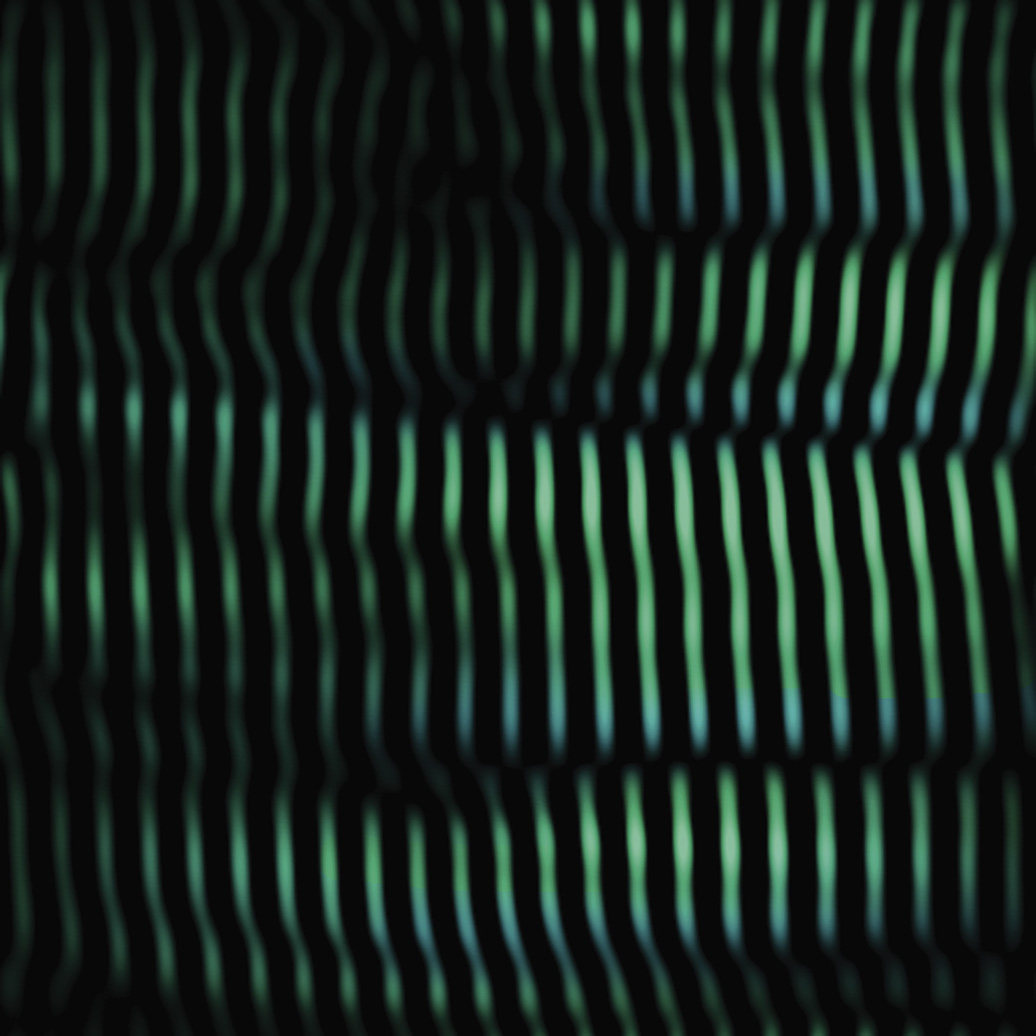
\includegraphics[width=1.0\linewidth]{chap4/4_0}
	% 加星号(*)表示不加编号
	\caption*{ \label{fig:4_0}}
\end{figure}


伦敦皇家学会拥有350年的历史,拥有近200年的传统,每年都会邀请科学家进行公开演讲,并经常进行一些简单的实验。
1952年,其中一项实验成为了热议话题。


两辆固定自行车朝向相反,并通过一条链条连接在一起,当一辆自行车向前踩踏板时,另一辆自行车的踏板就会向后移动(图~\ref{fig:4_1})。


\begin{figure}[!htb]
	\centering
	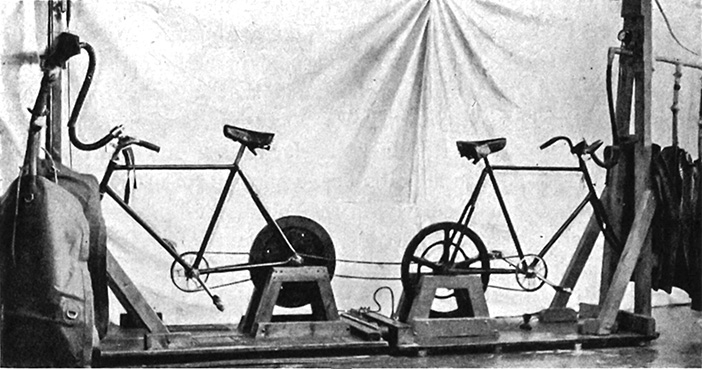
\includegraphics[width=1.0\linewidth]{chap4/4_1}
	\caption{Abbott 等人 (1952) 描述的推拉装置。 \label{fig:4_1}}
\end{figure}


一辆自行车上坐着一位娇小的女子,名叫布伦达$\cdot$比格兰,是肌肉疲劳研究领域的权威专家。
另一辆自行车上坐着一位魁梧的年轻人,名叫默多克$\cdot$里奇,他嫁给了他的自行车“对手”。
演讲者是A$\cdot$V$\cdot$希尔,他因在肌肉产热方面的研究而获得了诺贝尔奖。


里奇听从指令,用尽全力向前蹬,而比格兰则用力蹬着脚蹬,阻止他继续蹬。
想象一下,当观众看到这位娇小的女子轻而易举地阻止了这位身材高大的男人蹬得更快时,他们会有多么惊讶。
很快,他便大汗淋漓,气喘吁吁,而比格兰却几乎毫不费力。
甚至连伦敦市长后来也过来试驾。
“这套设备后来被命名为‘推拉你’,以纪念杜立特医生那只永远不知道自己要往哪个方向跑的双头怪兽,”布伦达$\cdot$比格兰-里奇后来写道。


魔术?小把戏?
并非如此,但它确实表明,肌肉消耗能量和产生力量的方式并非显而易见。
肌肉做正功(例如,在向前蹬踏时充当“马达”)时,它们消耗的能量和产生的热量,比做负功(例如,在向前蹬踏时充当“刹车”)时要多。
一般来说,肌肉产生的力量和消耗的能量,很大程度上取决于它是缩短还是伸长。
希尔实验的经验教训至今仍在日常康复和阻力训练中得到应用。
正如我们将看到的,奇迹发生在分子层面。


本章和下一章将深入探究肌肉内部,探索其结构与功能之间的关系。
肌肉是神奇的生物马达,能够在瞬间悄无声息地产生数千牛顿的力量。
这些力量如此巨大,以至于你小腿的肌肉就能举起一辆小型汽车的尾部。
这些巨大的力量是由数万亿个纳米级分子马达共同作用产生的,这些马达将我们摄入食物中的化学能转化为机械能,使我们能够活动。
这一非凡的功能源于骨骼肌特化的细胞机制和高度组织化的层级结构(图~\ref{fig:4_2})。


\begin{figure}[!htb]
	\centering
	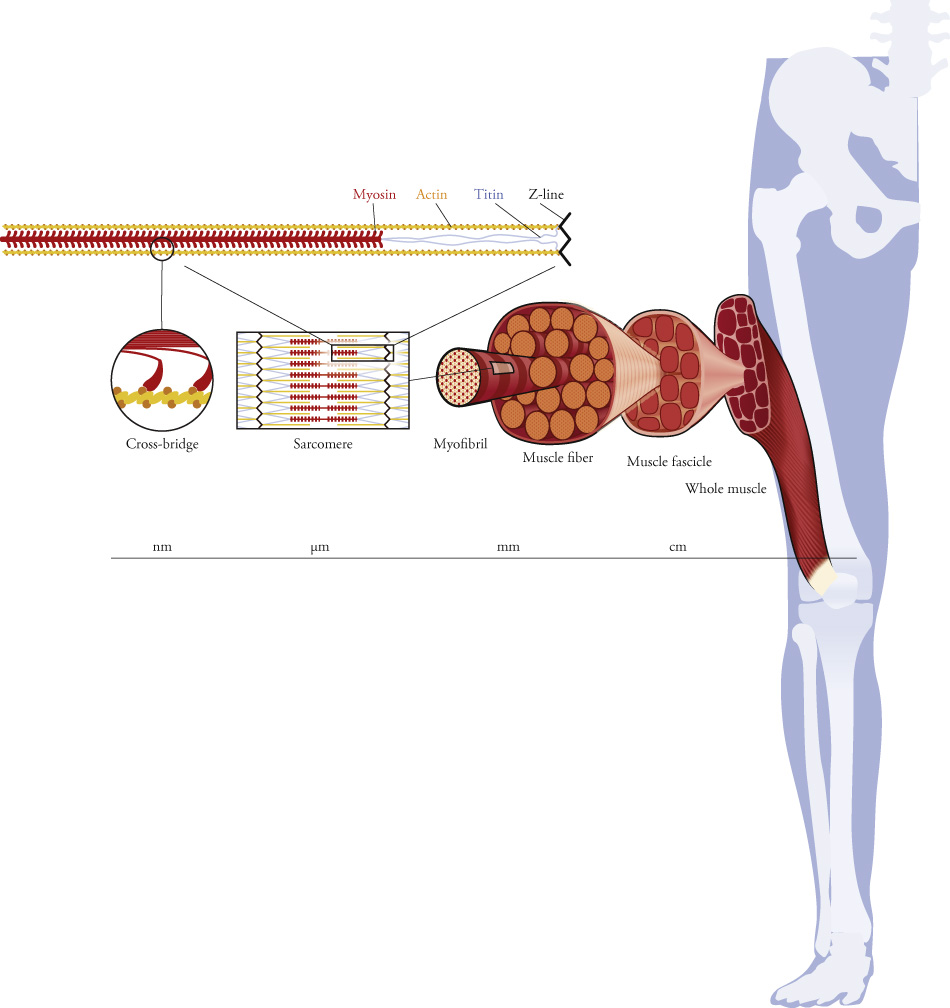
\includegraphics[width=1.0\linewidth]{chap4/4_2}
	\caption{肌肉的多尺度结构。
		骨骼肌具有层次结构,其中有被称为肌球蛋白的纳米级分子马达,每个肌球蛋白仅产生几皮牛顿的力,排列成肌节、肌原纤维、纤维、肌束和整个肌肉,在强力肌肉收缩期间可产生数千牛顿的力。 \label{fig:4_2}}
\end{figure}


接下来两章的组织将大致遵循肌肉的层级结构。
我们将首先在分子层面研究力量的产生过程。
接下来,我们将了解分子马达是如何被包裹在被称为肌节的亚细胞结构中的(活体人体肌节的第一张图像就是在我的手臂上拍摄的,并在本章的开篇图中展示)。
进一步深入,我们将了解单个肌肉细胞如何被神经系统激活,并了解“快肌纤维”和“慢肌纤维”之间的区别。
在第~\ref{chap:chap5}~章中,我们将从宏观层面研究肌肉在体内的排列方式,以及它们如何与肌腱(将肌肉力量传递到骨骼结构)相互作用。


\section{肌肉结构}

从最基本的层面来说,肌肉通过两种细长蛋白质(肌动蛋白和肌球蛋白)的相互作用产生力量。
20 世纪 50 年代初,休$\cdot$赫胥黎通过 X 射线显微镜发现,这些蛋白质平行排列,纤维交织,它们之间的连接被他称为“横桥”。
安德鲁$\cdot$赫胥黎(与休无亲属)同时用不同的方法发现了横桥。
休$\cdot$赫胥黎和安德鲁$\cdot$赫胥黎都怀疑横桥是产生力量的机制,并于 1954 年提出了一个关于这些分子马达如何工作的模型,我们将在下文中解释。
他们的模型一直是解释力量产生的基本范式,尽管随着更多实验数据的收集,该模型变得更加详细。


从尺寸上看,肌纤维排列成束,称为肌束,它们与肌肉纤维一样,长度可达数十厘米。
肌束的横截面积约为 1 毫米。
除了肌纤维外,肌束还包含称为细胞外基质的结缔组织,其中包括胶原蛋白、神经纤维和血管。
在健康的肌肉中,肌纤维紧密排列;
然而,在患病的肌肉中,肌纤维的横截面积可能较小,并被更多的细胞外基质和脂肪隔开。


肌束被更多结缔组织包围,并聚集在一起形成肌肉。
另一层结缔组织鞘被称为筋膜,包裹着肌肉并将其与其他肌肉隔开。
终止于每个肌束末端的肌纤维可以直接附着在骨骼上,但通常它们会连接到肌腱,肌腱随后附着在骨骼上。
肌腱插入肌肉的部分称为腱膜;
肌腱在肌肉外部的部分通常称为游离肌腱。
正如我们将在第~\ref{chap:chap5}~章中看到的,肌腱不仅通过向骨骼传递肌肉力量发挥着重要作用,还在伸展和回缩时储存和释放能量。


\section{横桥循环}

当神经系统激活肌肉时,肌肉会通过数万亿个肌动蛋白和肌球蛋白的协同作用产生力量,这个过程被称为“横桥循环”(图~\ref{fig:4_3})。
这种机制可以粗略地描述为一个分子大小的棘轮。


\begin{figure}[!htb]
	\centering
	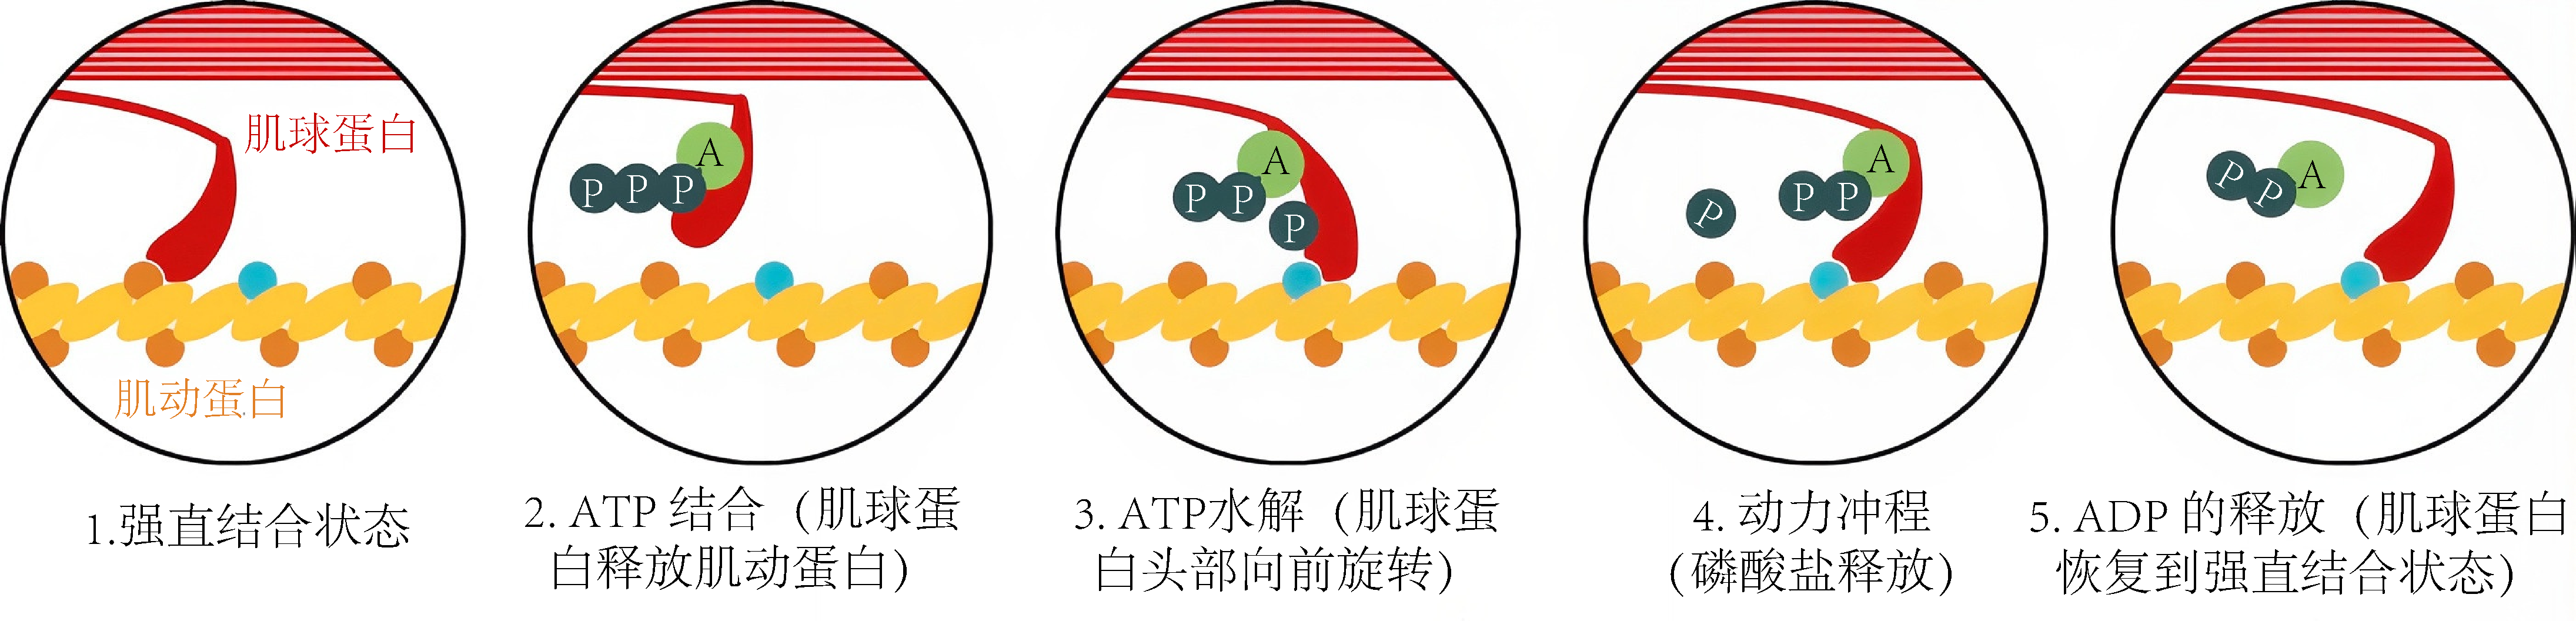
\includegraphics[width=1.0\linewidth]{chap4/4_3}
	\caption{横桥循环描述了肌动蛋白和肌球蛋白相互作用产生力量和运动的过程。
		A 代表腺苷;P 代表磷酸。 \label{fig:4_3}}
\end{figure}

肌球蛋白分子分为 3 个区域,分别称为头部、颈部和尾部。
肌球蛋白头部的独特结构使其能够牢固地结合到肌动蛋白丝上的特定位置(图~\ref{fig:4_3}~第一帧)。
当肌肉需要产生力量时,肌球蛋白头部会接收一种名为三磷酸腺苷 (ATP) 的“燃料”分子。
这刺激肌球蛋白头部从肌动蛋白上分离,向前旋转,并附着到肌动蛋白上的下一个结合位点(图~\ref{fig:4_3}~第二帧和第三帧)。
接下来,肌球蛋白头部围绕颈部区域旋转,这一运动被称为动力冲程 (power stroke),产生几皮牛顿的力,并使肌动蛋白丝彼此滑动约 10 纳米。


当然,不消耗能量就不可能完成机械功。
能量来自于一个化学反应,该反应将一个磷酸离子从三磷酸腺苷中分离出来(图~\ref{fig:4_3}~中的图4),留下二磷酸腺苷(ADP)。
最终,二磷酸腺苷被释放,肌球蛋白恢复到其原始状态,但现在已从其原始位置移位。
当肌球蛋白以这种方式循环时,细丝被拉向肌节中部,从而在化学能转化为机械能的过程中产生张力。


虽然这种机制听起来可能很复杂,但它却是一个优雅而经济的解决方案,解决了如何在分子层面上以可预测的方向产生力的问题。
就像汽车发动机一样,我们的肌肉将化学能转化为机械能,但噪音更小,产生的有毒废气也更少。



\section{肌节结构}

再往上一层,我们来看看肌节。
肌节大致呈圆柱形,长度根据肌肉长度在 1 微米到 5 微米之间变化。
肌节由许多相互交织的“粗”肌丝和“细”肌丝组成,随着肌节长度的变化,这些肌丝会相互滑动。


数百条肌球蛋白尾部捆绑在一起,形成每根粗肌丝,形成棒状结构,肌球蛋白头部以规则的间隔向外放射状延伸(图~\ref{fig:4_4})。
与粗肌丝平行的是细肌丝,它们由 3 种蛋白质组成:
肌动蛋白、原肌球蛋白和肌钙蛋白。
我们已经描述了肌动蛋白,它为肌球蛋白头部提供结合位点。
这些结合位点沿着细肌丝以规则的间隔分布。
原肌球蛋白和肌钙蛋白仅在肌肉被神经系统激活且存在钙离子时才会暴露这些结合位点,从而帮助调节力量的产生。
另一种值得关注的蛋白质(肌联蛋白),将每根粗肌丝附着在肌节的末端(我们称之为 Z 线或 Z 盘)。
正如我们稍后将看到的,肌联蛋白在被动力的产生中起着重要作用,这是一个独立于横桥循环的过程,也是赫胥黎最初的模型所忽略的现象。

\begin{figure}[!htb]
	\centering
	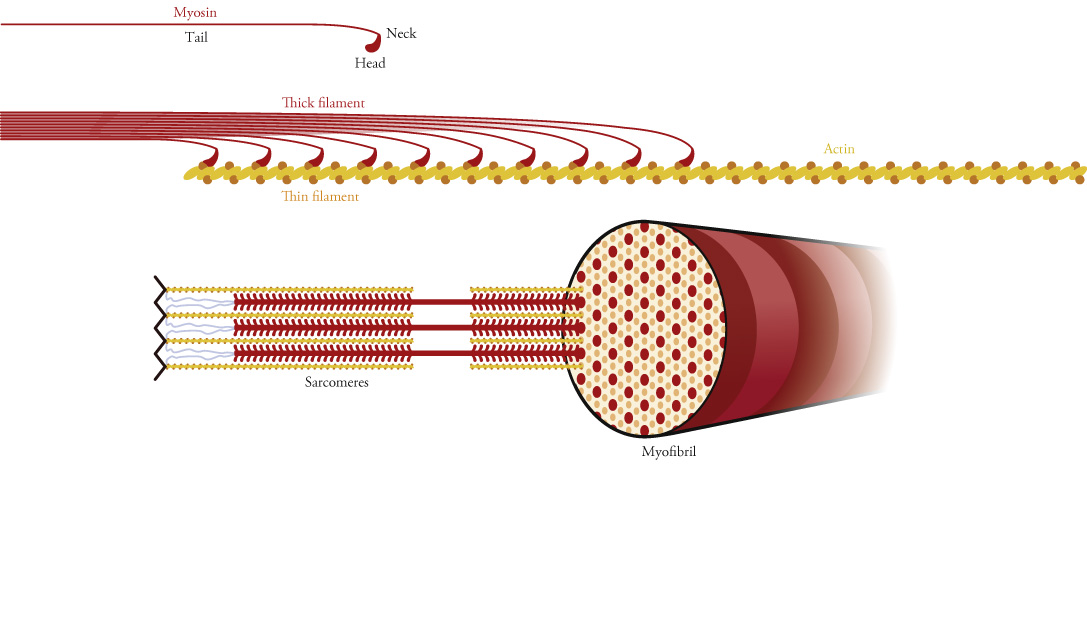
\includegraphics[width=1.0\linewidth]{chap4/4_4}
	\caption{肌球蛋白示意图(顶部)、粗丝和细丝的相互作用示意图(中间)以及肌原纤维横截面,显示粗丝和细丝以高度有序的三维模式排列(底部)。 \label{fig:4_4}}
\end{figure}

肌节在骨骼肌内以规则的模式串联和平行排列,在显微镜下观察骨骼肌组织时,会形成条纹,即明暗交替的带状结构。
您可以在图~\ref{fig:4_5}~中看到这些带状结构,它们分别被称为 I 带、A 带、Z 盘和 M 盘。
严格来说,Z 盘和 M 盘确实是圆盘,但它们通常被称为 Z 线和 M 线,因为它们在二维空间中看起来是这样的。
A 带仅出现在含有肌球蛋白的区域,而 I 带则出现在其他区域。细肌动蛋白丝的一端锚定在 Z 盘上。
粗肌球蛋白丝的一端附着在 M 盘的结构上,另一端通过肌联蛋白分子固定在 Z 盘上。
骨骼肌有时被称为“横纹肌”,与“平滑肌”相对,例如控制血管口径的肌肉,它们没有组织成肌节,也没有呈现条纹图案。

\begin{figure}[!htb]
	\centering
	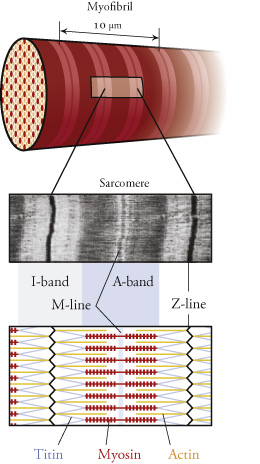
\includegraphics[width=0.5\linewidth]{chap4/4_5}
	\caption{肌原纤维示意图(上)展示了其高度组织化的微观结构。
		肌肉显微镜图像(中)和肌节示意图(下)分别标记了I带、A带、M线和Z线。
		肌节的末端由Z线定义。 \label{fig:4_5}}
\end{figure}


\section{力-长度关系}

肌节所能产生的最大力量会随着其长度的变化而变化。
长度和张力之间的关系可以用滑动丝理论来解释,该理论由两个研究小组于 1954 年独立提出。
Andrew Huxley 和 Rolf Niedergerke(在单根肌纤维中)以及 Hugh Huxley 和 Jean Hanson(在分离的肌原纤维中)证明,在主动肌肉收缩过程中,肌小节带不会变窄,这推翻了粗肌丝缩短的流行理论。
他们给出的解释是,随着肌节长度的变化,粗肌丝和细肌丝会相互滑动。
因此,肌节的长度会影响肌动蛋白和肌球蛋白之间“重叠”的量,或者说靠近细肌丝上结合位点的肌球蛋白头部的数量。
随着肌球蛋白头部和肌动蛋白结合位点之间横桥数量的增加,激活的肌节内的张力也会增加。


如图~\ref{fig:4_6}~所示,激活的肌肉中横桥循环所能产生的力随肌节长度而变化。
该主动力-长度曲线通常被描述为具有三个区域:
上升区,其中力随肌节长度的增加而增加;
平台区,其中力保持在最大值;
下降区,其中力随肌节长度的增加而减小。
平台区涵盖一系列肌节长度,称为“最佳”范围,其中肌球蛋白头部和肌动蛋白结合位点之间的相互作用数量达到最大值。
最佳肌节长度因脊椎动物而异,但通常在 2.2 至 2.7 μm 之间,在人类骨骼肌中约为 2.7 μm。
当肌节长度超过最佳范围时,肌动蛋白和肌球蛋白的重叠量会减少,横桥循环所能产生的力量也会减少。
当肌节长度略短于最佳长度时,源自肌节两端的细肌丝开始在肌节中部重叠并相互干扰,导致所谓的“浅上升区”的力量减弱。
当肌节长度更短时(在“陡峭上升区”),粗肌丝会与Z盘碰撞并变形,产生阻碍横桥循环作用的力量。
由于肌肉由串联和并联排列的肌节组成,我们可以观察到肌肉主动收缩过程中力量与长度之间的类似关系。

\begin{figure}[!htb]
	\centering
	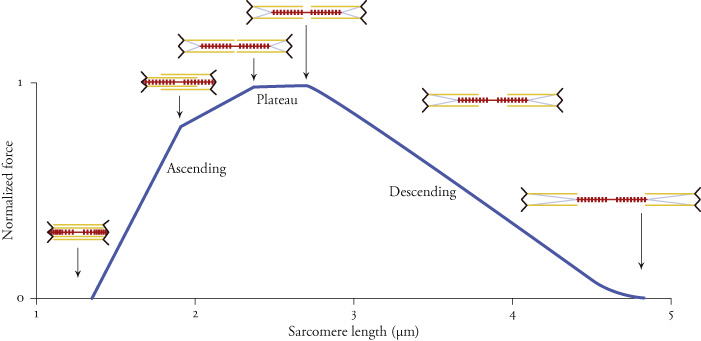
\includegraphics[width=0.5\linewidth]{chap4/4_6}
	\caption{肌节产生的主动力与其长度有关。粗肌丝和细肌丝相互滑过时,力会发生变化。
		在肌节的上升支,力随长度增加而增大,达到平台期;
		在肌节的下降支,力随长度增加而减小。
		当横桥数量达到最大时,力的产生达到峰值\cite{gordon1966variation}。 \label{fig:4_6}}
\end{figure}


即使在不活动时,肌肉在拉伸超过其静息长度时也会产生力,就像非线性弹簧一样。
这种被动力-长度关系主要源于肌肉中的两种结构:肌联蛋白以及围绕纤维、肌束和肌肉的结缔组织。
肌联蛋白是一种大型、柔韧的蛋白质,它将粗肌丝固定在肌节两端的Z形盘上。
当肌节较短时,肌联蛋白呈卷曲状,刚度较低;随着肌节变长,肌联蛋白变直,刚度增加(图~\ref{fig:4_7})。
肌纤维周围的结缔组织也表现出类似的力-长度行为。肌肉激活时产生的总力是其被动力与横桥产生的主动力之和(图~\ref{fig:4_8})。

\begin{figure}[!htb]
	\centering
	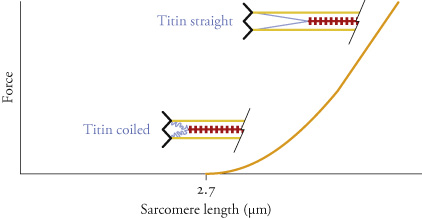
\includegraphics[width=0.7\linewidth]{chap4/4_7}
	\caption{肌联蛋白将粗肌丝附着在肌节两端的 Z 盘上,并在拉伸时产生力量。 \label{fig:4_7}}
\end{figure}

\begin{figure}[!htb]
	\centering
	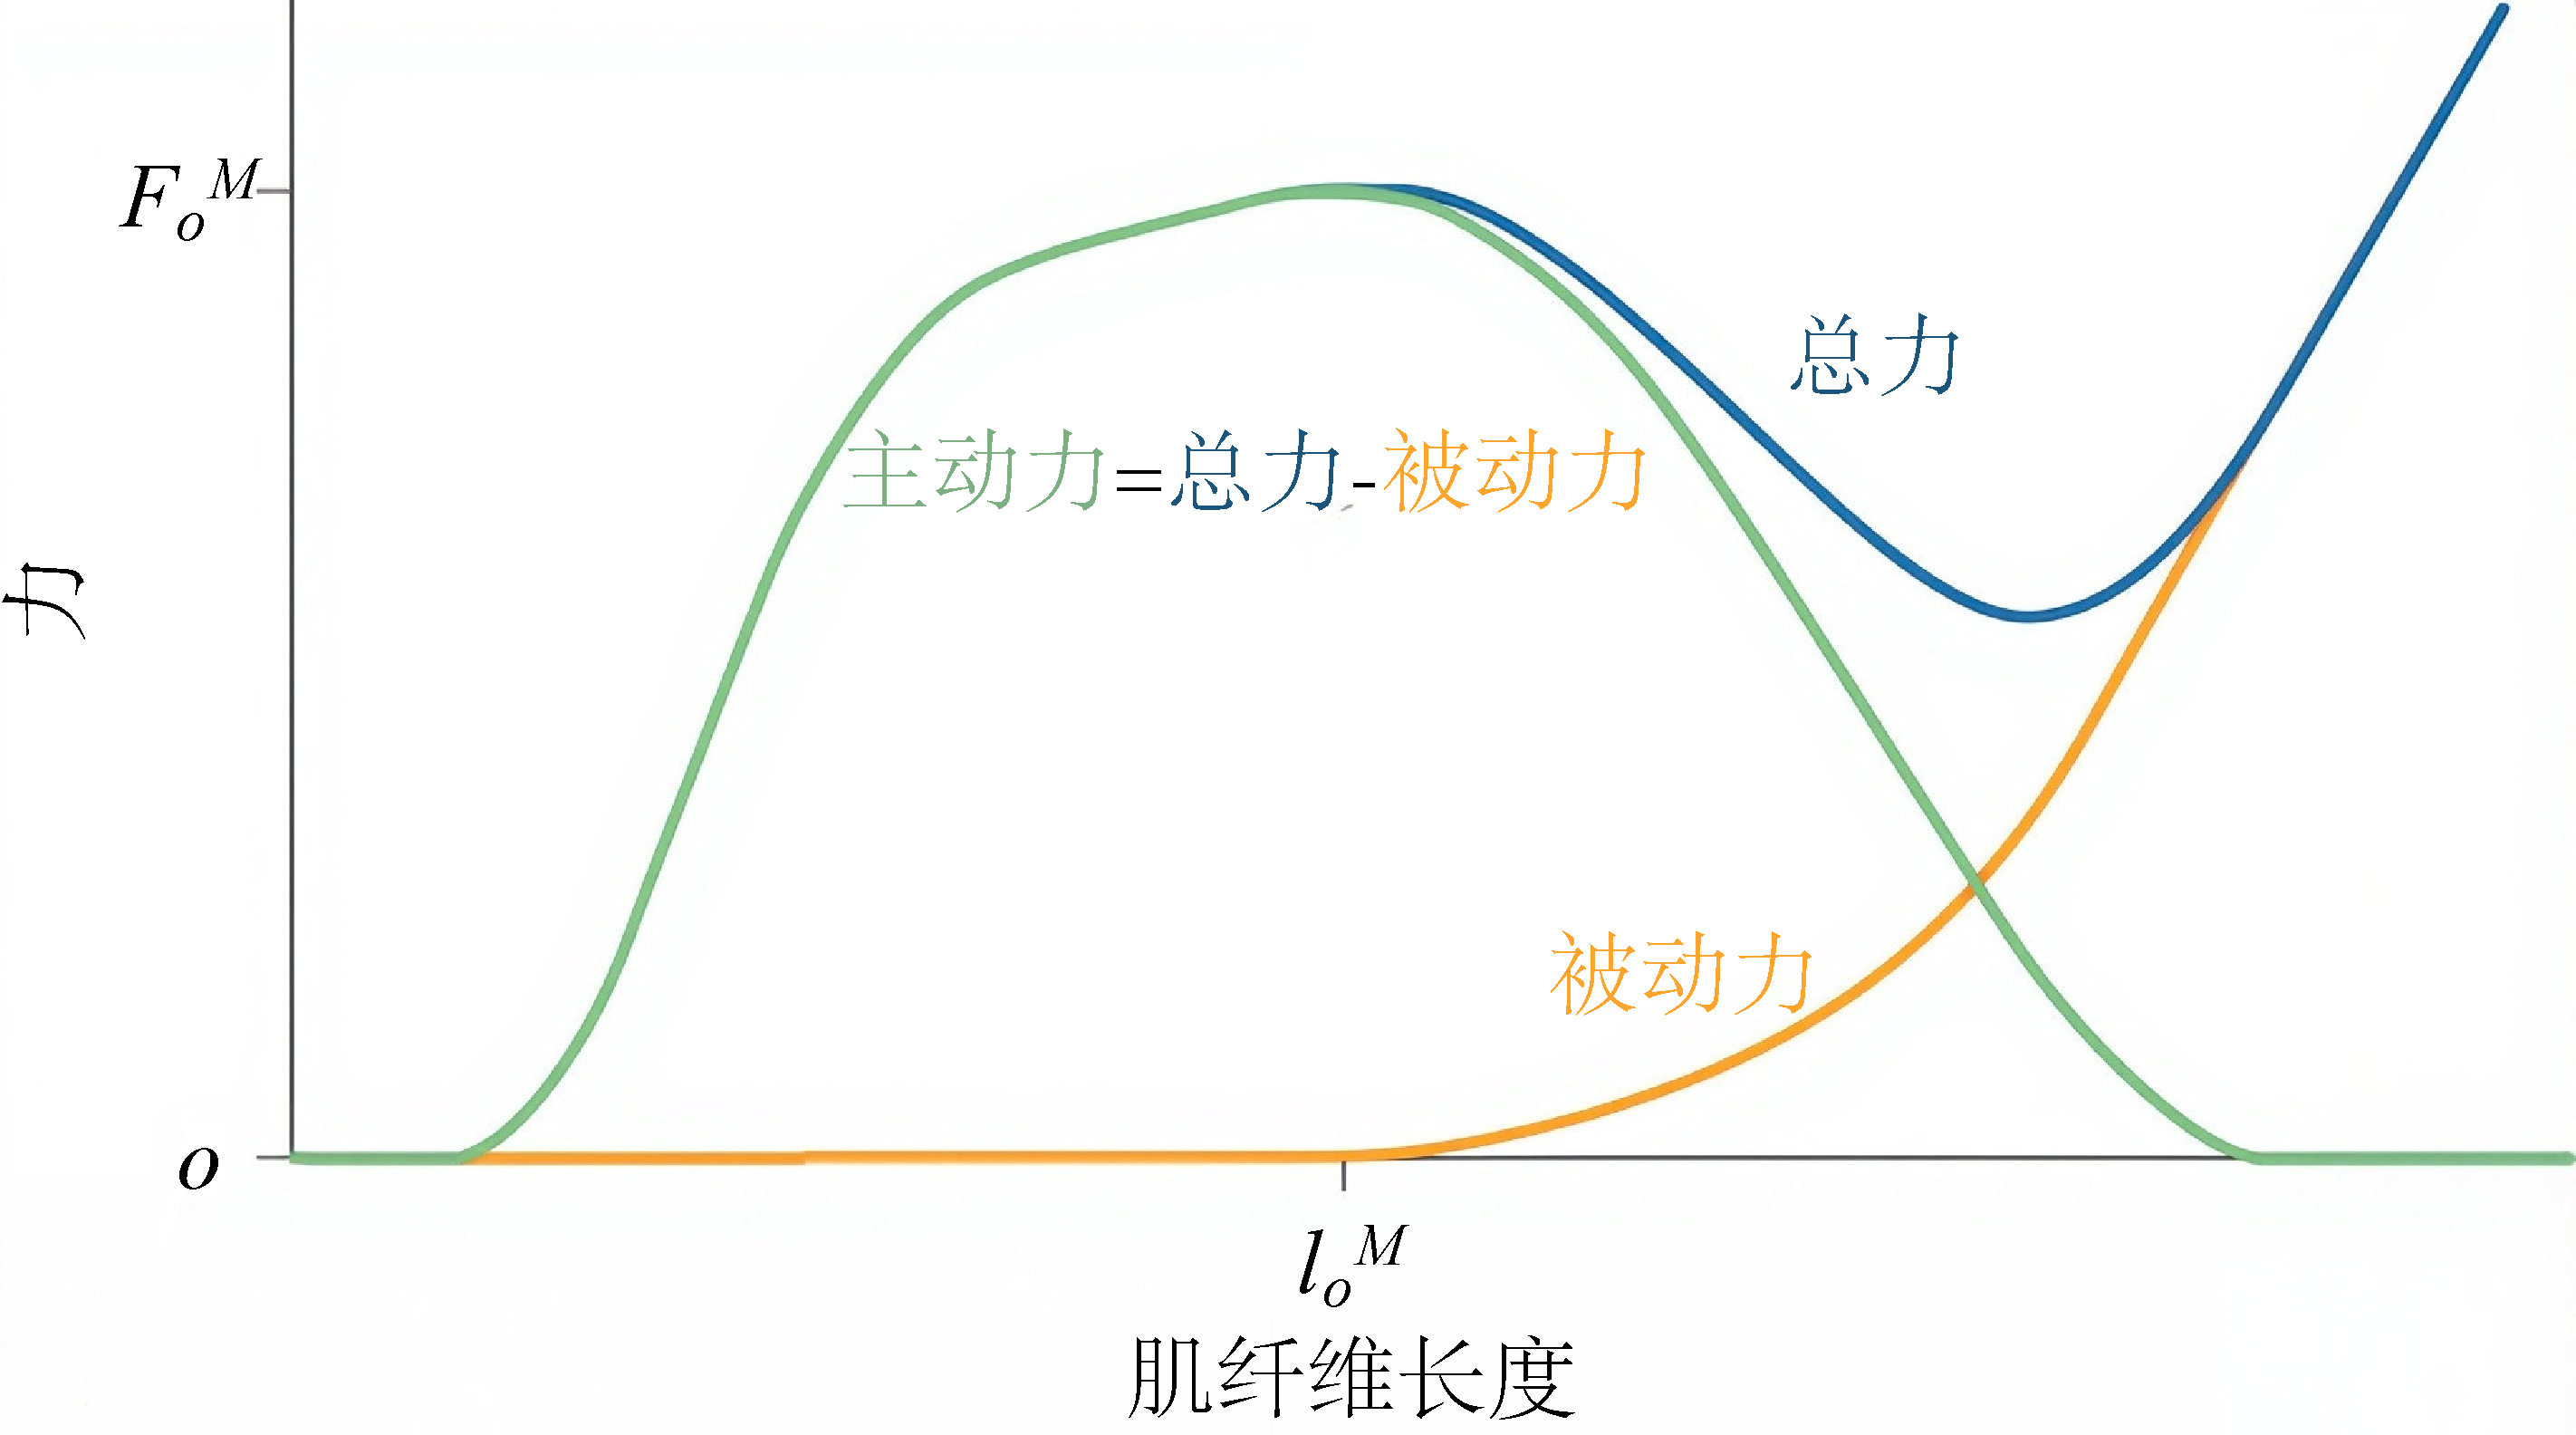
\includegraphics[width=0.7\linewidth]{chap4/4_8}
	\caption{主动力-长度曲线可以通过从一系列纤维长度的总力中减去被动力的测量值来确定。
		峰值主动力 $F_o^M$ 出现在最佳肌纤维长度 $l_o^M$ 处。 \label{fig:4_8}}
\end{figure}


\section{力与速度的关系}

肌肉产生的力量不仅取决于其长度,还取决于其长度变化的速率,这一点可能会让人感到惊讶。
我们用力-速度曲线(图~\ref{fig:4_9})来描述这种速率依赖性。
这种关系最早由A. V. Hill于1938年观察到,并最终促使他和他的同事们开发了本章开头描述的“推我拉你”实验。

\begin{figure}[!htb]
	\centering
	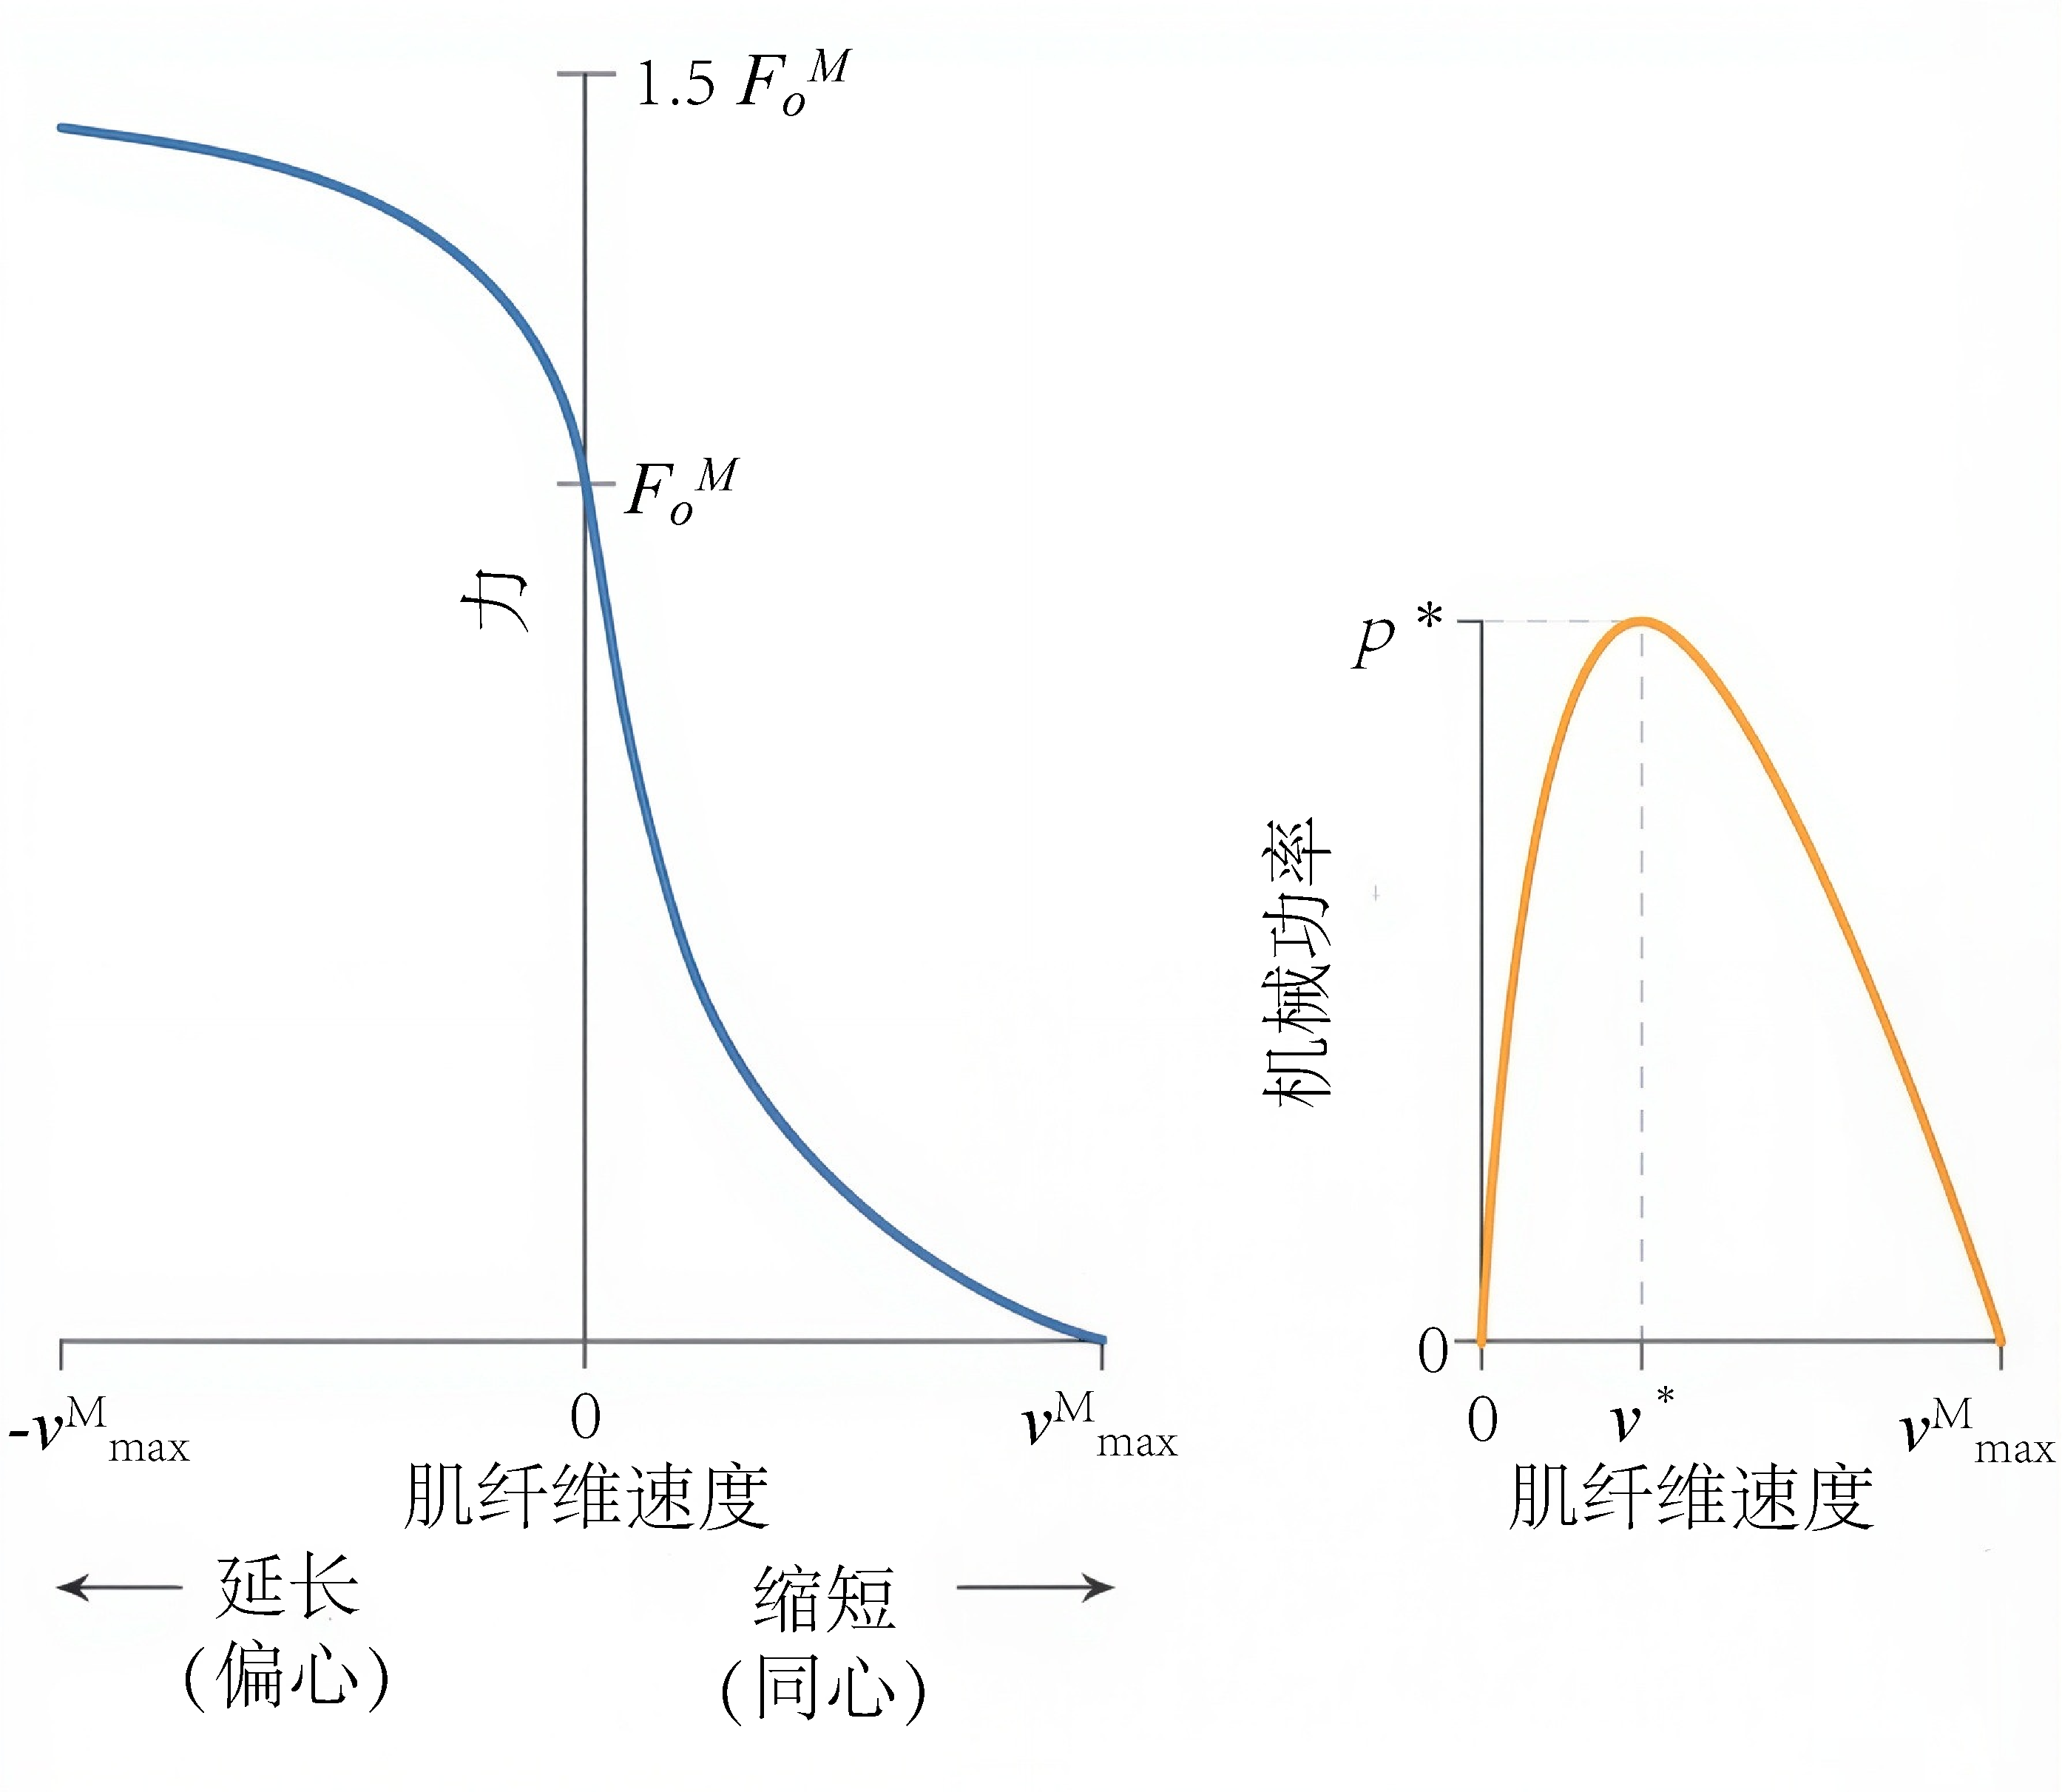
\includegraphics[width=0.7\linewidth]{chap4/4_9}
	\caption{肌纤维力和功率是肌纤维速度的函数。
		肌纤维伸长时,力产生能力增加;缩短时,力产生能力降低(左)。
		机械功率是力与速度的乘积,在最大缩短速度($v^*$;右)的约三分之一处达到最大值($p^*$)。 \label{fig:4_9}}
\end{figure}

力量取决于速度的原因如下。
肌节通过横桥循环产生力量,在此过程中,肌球蛋白头部与肌动蛋白丝结合并对其施加拉力。
由于此过程需要时间,因此当肌节缩短时,通过横桥循环产生的主动力会减小。
在非常高的缩短速度下,由于粗肌丝和细肌丝相互滑动的速度快于肌球蛋白头部在动力行程中旋转的速度,因此无法产生主动力。
相反,当肌肉拉长时,主动力会增加,因为肌球蛋白的颈部区域在头部与细肌丝分离之前会受到拉力。
非常高的拉长速度会损伤这些结构和其他结构,导致肌肉主动力急剧下降。


肌肉的速度在锻炼时至关重要。
在等长运动中,肌肉在受到相等阻力时被激活。
在这种情况下,肌肉的长度不会改变(即速度为零)。
如果肌肉受到的阻力较小,肌肉就会缩短,这种收缩被称为向心收缩。
相反,如果肌肉受到的阻力较大,肌肉就会伸长,这种收缩被称为离心收缩。


希尔观察到,在向心收缩过程中,随着缩短速度的增加,主动力呈双曲线下降,在最大收缩速度($v_{\text{max}^M}$)时达到零。
在离心收缩过程中,肌肉力量超过其等长收缩过程中的力量,最高可达其最大等长力量的1.5倍左右。


希尔的观察解释了为什么默多克$\cdot$里奇在“推我拉你”实验中费力不讨好,而布伦达·比格兰却几乎不费吹灰之力。
该装置迫使里奇的肌肉在图~\ref{fig:4_9}~中“向心”一侧运作,此时它们施加的力量远低于其最大力量。
相比之下,比格兰的肌肉则在力-速度曲线的“离心”一侧运作,此时它们几乎可以施加其最大力量。
里奇向前蹬踏,就像发动机一样,而比格兰向后蹬踏,就像刹车一样。


向心收缩和离心收缩的另一个区别在于肌肉所做功的性质。
向心收缩时,肌肉做正功,因为力和位移的方向相同。
然而,离​​心收缩时,肌肉也做功(即肌肉做功为负),因为力和位移的方向相反。


你可能想知道,在日常生活中,肌肉是否同时做正功和负功。
确实如此!骑车或步行上坡时,你的肌肉主要做正功。
然而,当你走下陡坡时,你的许多肌肉会做负功来控制下坡速度。
有趣的是,做负功会使肌肉酸痛,并促进肌肉再生。


负功理论认为,肌肉理论上可以从外力中获取能量或“充电”。
可惜,这根本不可能发生。
我们的身体无法逆转驱动横桥机制的化学反应,将二磷酸腺苷(ADP)转化回三磷酸腺苷(ATP)。
然而,对于由可充电电池驱动的机器来说,充电是可能的。
例如,传统汽车的摩擦制动器将动能转化为热能,而电动汽车则利用再生制动来捕获和储存这种能量。


力-速度关系对收缩肌肉产生的机械功率有重要影响(图~\ref{fig:4_9},右图)。
当肌肉等长收缩时,可以产生很大的力,但速度为零;
因此,作为力和速度的乘积的机械功率为零。
在缩短速度 及以上时,机械功率也为零,此时速度很大,但不会产生力。
峰值正机械功率出现在大约 $v_{\text{max}^M}$ ,此时力和速度的乘积达到最大值。
功率-速度关系可以很好地预测日常运动的一些特征。
例如,当骑自行车的人感觉到他们的肌肉移动得太快或太慢时,他们就会换挡,远离最大功率范围。


\section{肌肉激活}

我们假设,只要肌球蛋白头部靠近细丝上的结合位点且存在ATP,肌动蛋白和肌球蛋白就能进行横桥循环。
然而,当肌肉放松时,肌动蛋白上的肌球蛋白结合位点会被原肌球蛋白阻断。
当肌肉兴奋时,钙离子被释放到细胞内空间并与蛋白质复合物肌钙蛋白结合,这会导致原肌球蛋白变形,暴露出细丝上的结合位点(图~\ref{fig:4_10})。


\begin{figure}[!htb]
	\centering
	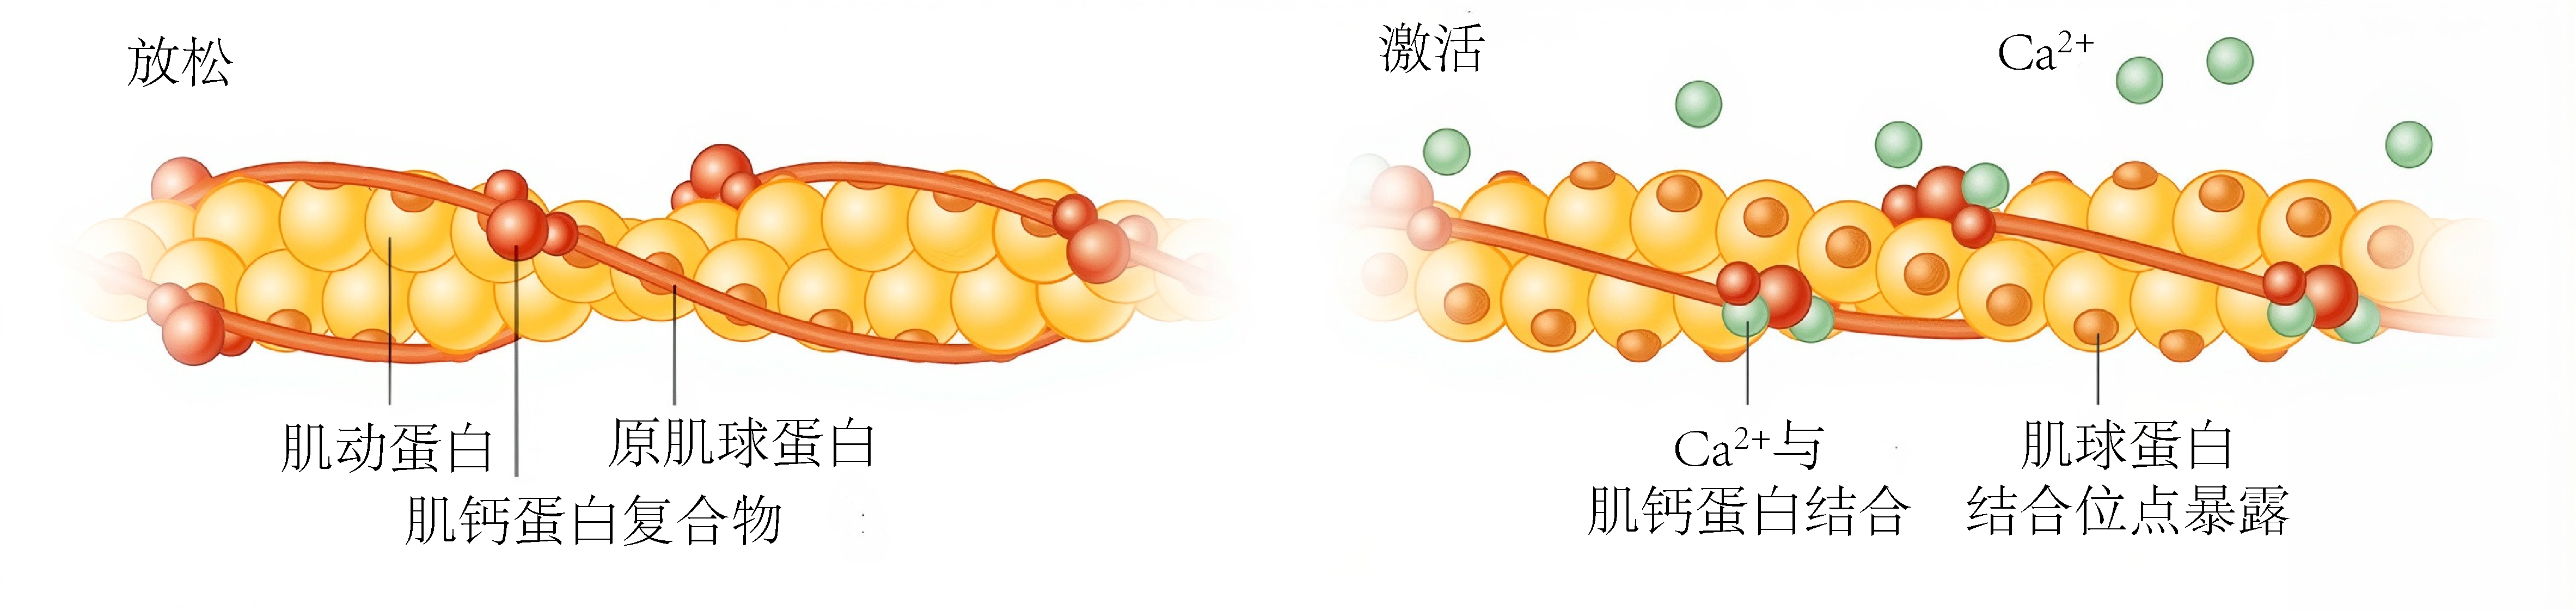
\includegraphics[width=1.0\linewidth]{chap4/4_10}
	\caption{肌肉激活过程中的分子变化。
		当肌肉放松时(左图),肌动蛋白丝上的肌球蛋白结合位点被原肌球蛋白阻断。
		肌肉激活(右图)会导致肌浆网释放钙离子。
		钙离子与肌钙蛋白复合物结合,导致原肌球蛋白变形,露出肌动蛋白上的肌球蛋白结合位点,从而允许横桥循环开始并产生力量。 \label{fig:4_10}}
\end{figure}

人们不禁会想:钙离子从何而来?
如前所述,它们储存在细胞内一种类似储罐的地方。
它们的释放由中枢神经系统(CNS)控制,它是肌肉发展过程中极其重要的一个环节,我们之前还没有提到过。
肌肉不会自行激活;通常情况下,它们只有在神经系统发出指令时才会活动。


肌纤维具有多种结构特征,使其能够接收来自中枢神经系统(CNS)的信号,并快速传播这些信号,从而沿着整个细胞释放钙离子。
运动神经元通过一个称为神经肌肉接头(neuromuscular joint)的特殊突触与每根肌纤维连接(图~\ref{fig:4_11})。
来自中枢神经系统(CNS)的兴奋信号会导致一种名为乙酰胆碱的神经递质跨神经肌肉接头突触转移。
这种转移触发细胞膜去极化,并导致正钙离子从肌浆网流出。
横轴管系统(通常简称为 T 小管)确保去极化沿着整个肌纤维快速传播。
T 小管是由细胞膜(称为肌膜)在细胞内延伸,将膜状指状结构伸入细胞质时形成的。
终末池位于T小管附近,是肌浆网的延伸,负责储存钙离子。
当细胞去极化时,钙离子会被释放到细胞内,从而启动横桥循环。


\begin{figure}[!htb]
	\centering
	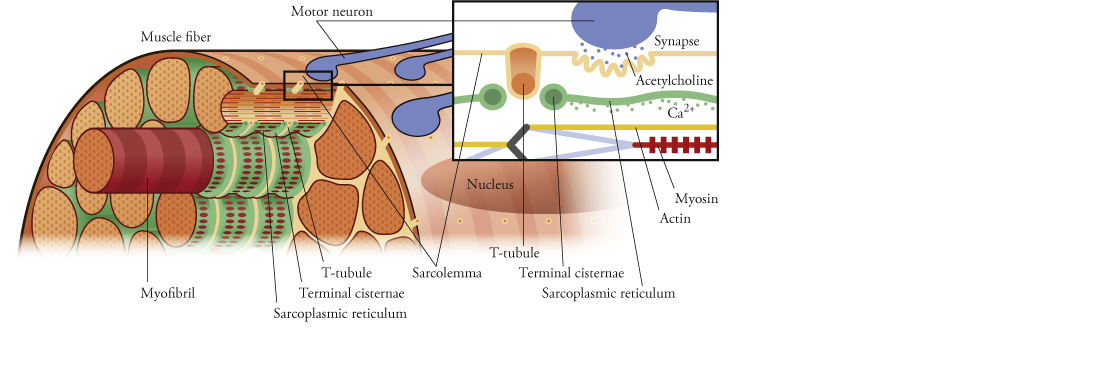
\includegraphics[width=1.0\linewidth]{chap4/4_11}
	\caption{肌纤维的结构使得动作电位能够快速传播,并协调整个长度上的横桥循环。 \label{fig:4_11}}
\end{figure}

当来自中枢神经系统的兴奋信号结束时,细胞开始将钙离子泵回肌浆网。
由于钙离子是逆浓度梯度运输的,因此钙离子的再吸收过程比释放过程慢。


到目前为止,我们仅研究了中枢神经系统如何激活肌肉。
但它的工作远未完成!它还需要告诉肌肉应该用力还是轻柔地拉动。
中枢神经系统利用上述机制,通过两种方式调节肌肉产生的力量:速率编码和运动单元募集。
我们将在接下来的两节中详细阐述这些机制。


\section{速率编码}

信息以电脉冲(称为动作电位)的形式在运动神经元中编码和传输。
通常,激活信号来自大脑,但也可以通过电流通过其支配的运动神经元来人工刺激肌肉。
功能性电刺激疗法利用了这一特性,通过电刺激脊髓损伤导致瘫痪的患者的外周运动神经元。
功能性电刺激系统可用于增强肌肉并产生协调运动,例如划船、抓握和骑自行车,正如我们在第一章中看到的。


对运动神经元施加短促的电刺激,只要刺激电压超过阈值,就会引起其所支配的肌纤维发生“抽搐”(图~\ref{fig:4_12})。
在电脉冲施加和力产生之间,存在一个短暂的延迟,因为去极化会传播并释放钙离子。
随后,纤维力迅速上升,达到峰值,然后相对缓慢地回落至零,因为再摄取过程会将钙离子泵出细胞内空间。


\begin{figure}[!htb]
	\centering
	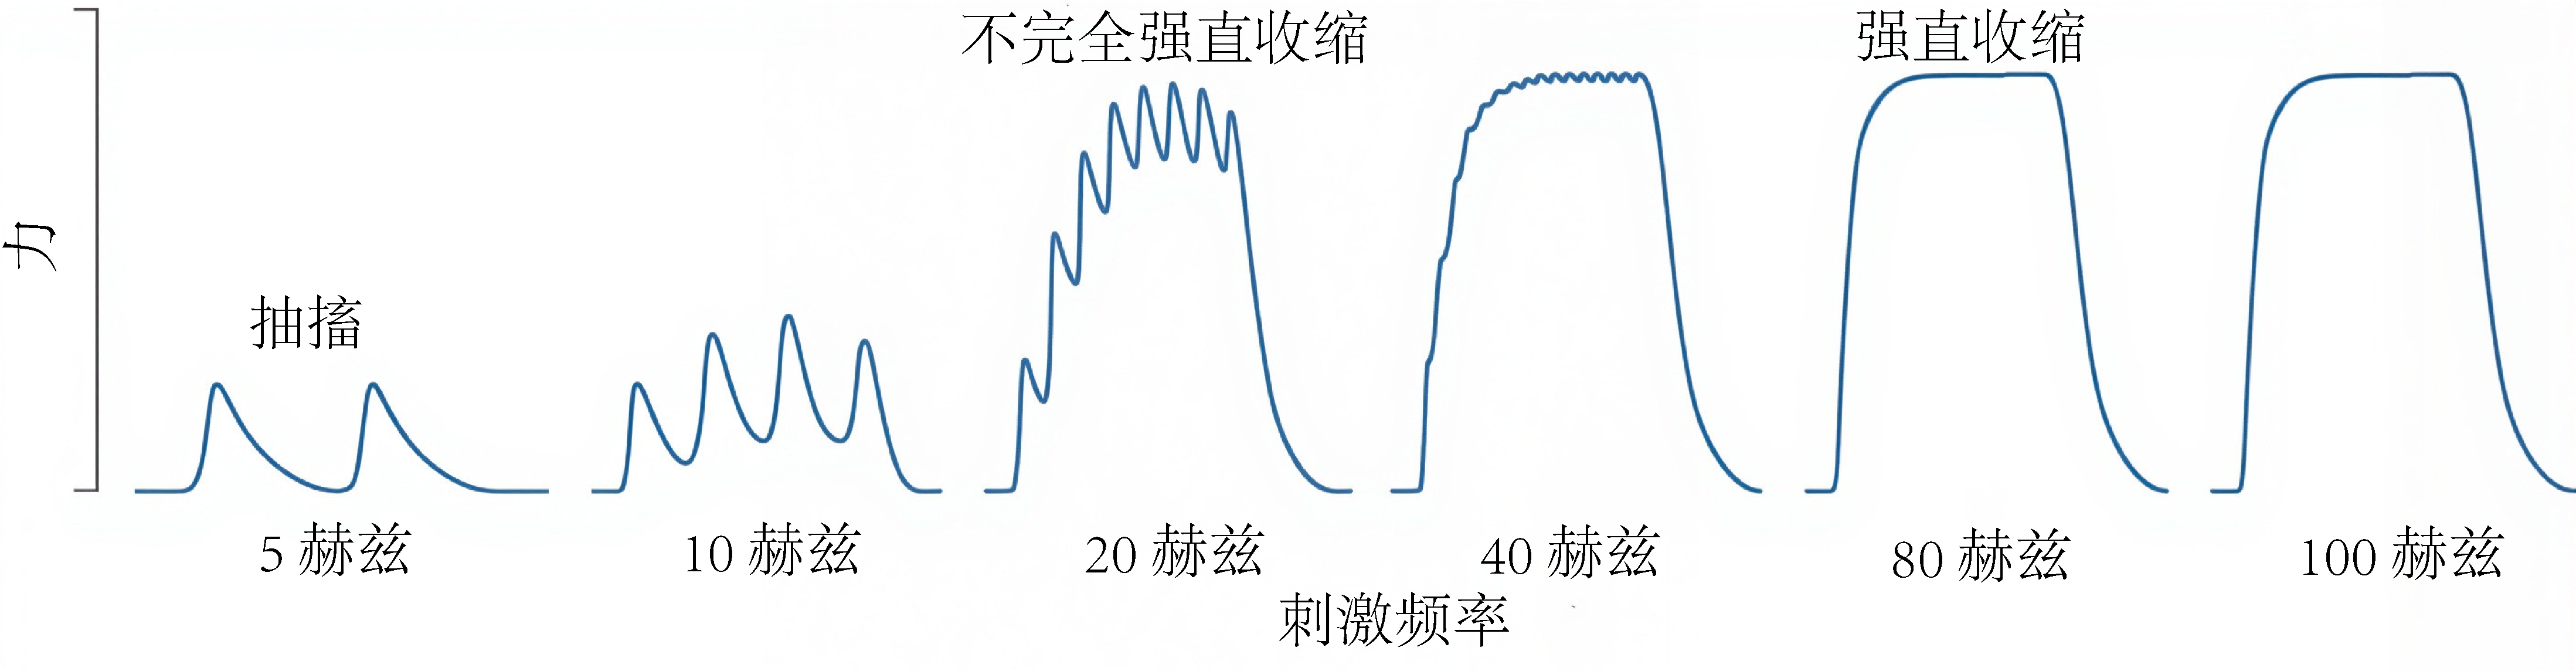
\includegraphics[width=1.0\linewidth]{chap4/4_12}
	\caption{不同刺激频率产生的肌肉力量。
		纤维力量受刺激频率(速率编码)调节,产生从抽搐(左)到融合性强直(右)的各种力量反应。 \label{fig:4_12}}
\end{figure}


刺激肌纤维通常不会使其产生单次抽搐;而是以特定速率施加一系列或一连串脉冲。
如果两次脉冲间隔足够近,第二次抽搐会在第一次脉冲的力完全衰减至零之前开始,从而产生高于第一次的第二个力峰值。
随着脉冲序列频率(或“发放频率”)的增加,峰值力也会增加——直到达到阈值刺激频率,此时纤维力达到稳定水平,峰值力在更高频率下不再增加。
该阈值刺激频率称为强直频率。
在强直频率或以上运作的肌肉被称为融合性强直(离散的抽搐融合在一起形成平滑的力分布);在较低频率下,肌肉被称为未融合性强直。
通过改变刺激频率,肌肉力可以从抽搐到强直进行大约四倍的调节。
换句话说,力的调节可以用刺激的速率来表示,因此称为速率编码。


当然,如果速率编码是调节力量产生的唯一机制,那么许多动作将无法实现。
许多肌肉需要超过四倍的力量变化才能完成其所需的功能范围,如果次最大肌肉力量像图~\ref{fig:4_12}~所示那样波动,我们的动作就会不稳定。


\begin{figure}[!htb]
	\centering
	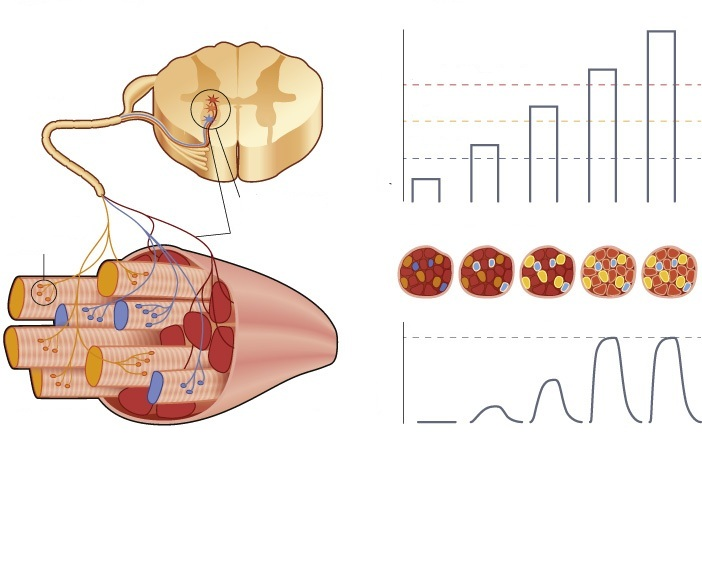
\includegraphics[width=1.0\linewidth]{chap4/4_13}
	\caption{运动单元募集。
		一个运动单元由一个运动神经元及其支配的肌肉纤维组成。
		图中显示了 3 个运动单元(蓝色、橙色和红色)(左图);
		中枢神经系统通过调节被募集的运动单元数量来调节肌肉力量(右图)。 \label{fig:4_13}}
\end{figure}


\section{运动单位募集}

正如预期,控制肌肉力量产生的第二种机制涉及调节控制信号的幅度,而不是频率。
神经系统通过只调动部分肌肉纤维来实现这一点,以完成任何给定的任务:产生较小力量时调动较少的肌肉纤维,产生较大力量时调动较多的肌肉纤维(图~\ref{fig:4_13})。
在次最大努力时,一些肌肉纤维处于非活动状态。


更详细地说,这个过程是这样运作的。
肌肉在功能上被划分为不同的运动单位,这些运动单位由一个运动神经元及其支配的肌纤维组成(图~\ref{fig:4_13},左图)。
运动单位的大小不一,从数十条肌纤维到数千条肌纤维不等。
需要精细控制的小肌肉,例如拇指肌肉,每个运动神经元仅包含少量肌纤维;而控制较粗略的大肌肉,例如背部肌肉,每个运动神经元则包含许多肌纤维。
通常,属于一个运动单位的纤维不会聚集在一起,而是分布在整个肌肉中。
因此,相邻的纤维通常属于不同的运动单位,并且由特定运动神经元支配的纤维可能位于多个肌束中。
中枢神经系统会根据任务需求调整被募集的运动单位数量(图~\ref{fig:4_13},右图)。


运动单元的募集遵循特定的顺序,称为有序募集,正如亨尼曼(Henneman)的尺寸原则\cite{henneman1965functional}所述。
为了产生较小的力量,中枢神经系统(CNS)仅募集小型运动单元。
随着所需肌肉力量的增加,中枢神经系统也会逐渐募集更大的运动单元。
小型和大型运动单元的区别不仅仅在于尺寸:优先募集的小型运动单元也更耐疲劳。
因此,在进行低强度运动时,中枢神经系统会选择性地募集小型纤维,以避免肌肉疲劳。
有序募集的重要性将在第~\ref{chap:chap5}~章中详细讨论。


与有序的运动单元募集不同,外部施加的电刺激并不会根据亨尼曼的大小原则募集运动单元。
当肌肉受到外部刺激时,大型运动单元会与小型运动单元同时被募集\cite{gregory2005recruitment}。
这对功能性电刺激具有重要意义。
尤其是在低水平刺激下募集大型易疲劳的纤维,会使其难以精确调节力量,并导致快速疲劳。


显然,如果我们能够在瘫痪患者中诱导有序募集,治疗质量将得到提升。
我实验室最近的实验表明,可以通过光学控制激活已改变为对光有反应的运动神经元,从而人工实现有序募集\cite{llewellyn2010orderly}。
这项技术最终可能为脊髓损伤和其他运动障碍患者带来更有效的疗法和治疗。



\section{肌电图}

当肌肉受到神经系统的刺激时,会产生一个微小的电信号。
我们刚刚看到,神经系统通过速率编码和运动单元募集来调节肌肉产生的力量。
粗略地说,通过运动神经元到达肌肉的刺激越大(无论是来自更高的频率还是更大的募集量),电信号就越大。
因此,我们可以使用肌电图 (EMG) 来测量肌肉活动水平,顾名思义,肌电图就是记录肌肉中的电活动。
如果我们将 EMG 电极连接到放大器和扬声器,我们就能听到肌肉的运动。
由于本书中我们会经常讨论使用 EMG 信号的研究,因此了解这些测量的基本原理非常重要。


为了记录肌肉活动,我们要么将电极贴到皮肤上进行“表面”肌电图,要么将导线插入肌肉进行肌内肌电图。
表面电极用于记录大块表层肌肉的活动,而肌内电极最适合较小或较深的肌肉。
在大多数设置中,每块肌肉使用一对电极(参考电极和信号电极);
因此,测得的时间序列代表肌肉内所有募集的运动单元的发放组合,并且可能包括周围的肌肉。
进一步复杂化地是,测量的幅度对电极相对于神经和肌肉纤维的位置很敏感(这可能难以精确控制,尤其是在运动过程中)。
因此,原始肌电图信号噪声很大,难以解释。


测量到的肌电信号通常会经过滤波和其他处理,以提高其可解释性(图~\ref{fig:4_14})。
我们通常对肌电信号进行高通滤波以消除随时间变化的漂移,然后对其进行整流和低通滤波,以获得一个包络,该包络可以指示肌肉活动幅度随时间的变化。
最后,我们根据在最大自主收缩或高强度动态运动期间收集的校准测量值对肌电信号进行归一化。
最终结果可以表示肌肉活动量占其最大值的百分比。


\begin{figure}[!htb]
	\centering
	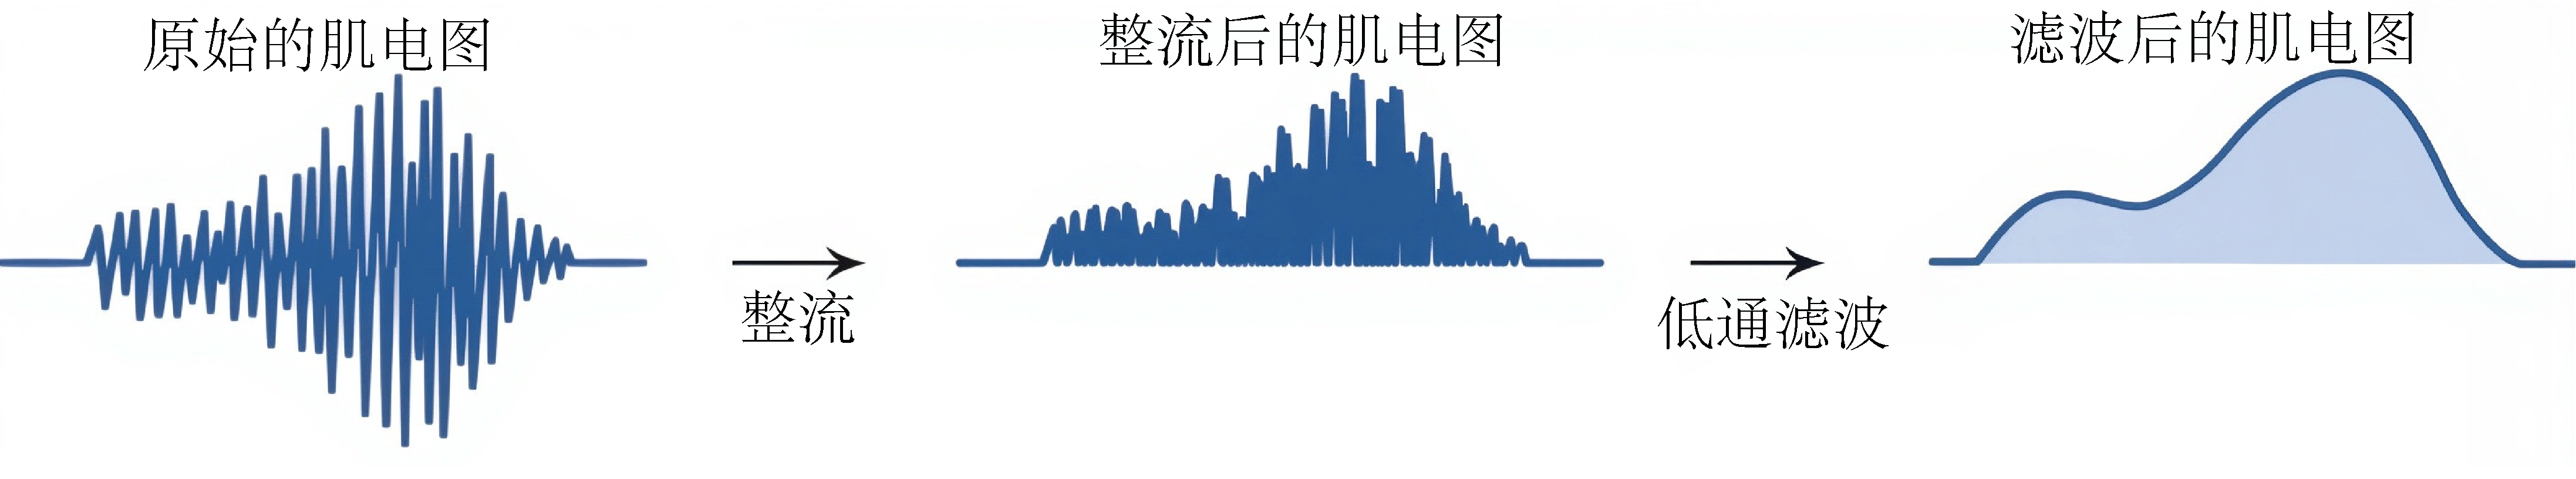
\includegraphics[width=1.0\linewidth]{chap4/4_14}
	\caption{肌电图 (EMG) 信号的处理。
		原始 EMG 信号的幅度会随着运动单元发放频率的增加和更多运动单元的募集而增大。
		为了便于解读,原始 EMG 信号通常经过高通滤波、整流、低通滤波,然后归一化至最大信号。 \label{fig:4_14}}
\end{figure}


在处理肌电图 (EMG) 信号时,通常会引入 2 种延迟,以将信号与肌肉的力量产生联系起来。
首先,非零肌电图 (EMG) 信号的出现和非零肌肉力量之间存在延迟;
延迟的持续时间可能因电极位置和肌肉种类而异。
第二个延迟是由于激活动力学造成的,如下所述。
肌电图 (EMG) 提供肌肉激活的总体测量,包括来自速率编码和肌肉募集的信息。
经过适当校准后,肌电图 (EMG) 可以成为研究肌肉协调性和测试肌肉激活模拟准确性的有用工具。


\section{肌肉激活动力学建模}

既然我们已经了解了一些肌肉生物学的基础知识,我们可以构建工程模型来描述肌肉力学。
为此,我们需要表征从肌肉兴奋到肌肉激活的转变,即所谓的激活动力学,并建立表示肌肉收缩动力学的方程(图~\ref{fig:4_15})。
下文我们将讨论激活动力学;收缩动力学将在下一章介绍。


\begin{figure}[!htb]
	\centering
	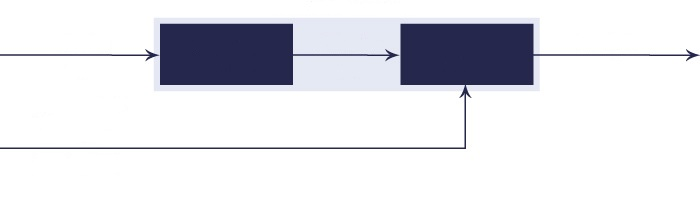
\includegraphics[width=1.0\linewidth]{chap4/4_15}
	\caption{肌肉-肌腱模型的输入和输出。
		在肌肉-肌腱执行器的计算模型中,我们假设激活动力学的过程(将激励 $(u(t))$  转换为激活 $(a(t))$)不同于收缩动力学,后者将肌肉-肌腱长度 $l^{\text{MT}(t)}$ 和速度 $v^{\text{MT}}(t)$ 与肌肉力 $F^{\text{M}}(t)$ 关联起来。 \label{fig:4_15}}
\end{figure}


速率编码和运动单元募集的影响可以纳入激活动力学的数学模型中。
肌肉激活的建模策略有很多;我的实验室采用以下方法。
该模型接受一个时变函数 $u(t)$ 作为输入,该函数描述了从神经到肌肉的兴奋信号强度。
其输出 $a(t)$ 是激活值,表示细胞内钙离子的可用性,从而表示横桥循环发生的程度。
$u(t)$ 和 $a(t)$ 均在 0(无兴奋;无横桥循环)和 1(最大兴奋;融合强直信号,所有运动单元均已募集)之间变化。


我们用经验确定的一阶常微分方程来模拟激发和激活之间的关系:
%
\begin{equation}
	\begin{aligned}
		\hat{a}(t) = \frac{u(t) - a(t)}{\tau} \\
		\text{其中,} \tau =
	\end{aligned}
\end{equation}


参数 A 和 D 分别表示激活和失活时间常数。
如上所述,A 小于 D;典型值分别为 10 毫秒和 40 毫秒,但这些值可能会随年龄、肌肉成分和其他因素而变化。
图~\ref{fig:4_16}~显示了当输入 $u(t)$ 为方波时,该微分方程的典型解。

\begin{figure}[!htb]
	\centering
	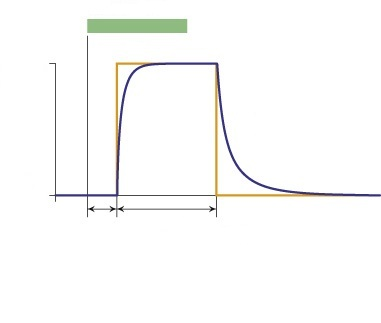
\includegraphics[width=1.0\linewidth]{chap4/4_16}
	\caption{激活动力学计算模型使用一阶常微分方程将激励 $(u(t))$ 与激活 $(a(t))$ 联系起来。
		激励通常滞后于测量的肌电信号,而力的产生则滞后更远。 \label{fig:4_16}}
\end{figure}


\section{力-长度-速度-激活关系建模}






